\documentclass[10pt,twocolumn]{article}

\usepackage{times}
\usepackage{spverbatim}
\usepackage[swedish]{babel}
\usepackage[utf8]{inputenc}
\usepackage{listings}
\usepackage[toc,page]{appendix}
\usepackage{graphicx}
\usepackage{mathtools}
\usepackage{float}
\usepackage[margin={2.45cm, 2.45cm}]{geometry}
\renewcommand\appendixname{Bilagor}
\renewcommand\appendixpagename{Bilagor}
\addto\captionsswedish{\renewcommand{\figurename}{Figure}}

\raggedbottom
\sloppy

\title{Parallelizing Mandelbrot set computation\\ TDDD56 }

\author{Martin Söderén \\ marso329, 9009291098 }

\date{\today}

\begin{document}

\maketitle

\clearpage

\section{Introduction}
This lab aims to implement two parallell algorithms that calculate the Mandelbrot set. For the complete definition of the Mandelbrot set see the lab description. Each complex number in the predefined set is calculated by iterating over it. If the computation reaches a maximal number of iterations the complex number is belived to be in the Mandelbrot set. If during the computation the series is detected to diverge then it is not belived to be in the set. 
\newline
\newline
Each computation for the complex number is independent so these can be calculated in parallel. This is called embarassingly parallel algorithm. For each complex number \textit{z} a point \textit{p} in a image is defined where the complex numbers real part is the position on the x-axis and the imaginary part is the position on the y-axis.  

\section{Method}
For the first part of the lab we are to implement a naive algorithm that just splits the image into equal part. This is not the best algorithm since calculating if a certain pixel is in the Mandelbrot requires the maximum number of iteration. Some threads will get more work than others if they get parts of the image that contains alot of pixels in the set. You can see the code for this implementation in appendix~\ref{app:naive} and the resuling image can be seen in figure~\ref{fig:naive}.
\newline
\newline
The second part of the lab is to the implement a better algorithm that has some kinde if loadbalancing. This was achieved by splitting the image in a 10x10 grid and having a counter protected by a mutex lock that counts up when a worker thread starts working on a part of the grid. From this number each thread can calculate which pixels should be calculated.  The code for this implementation can be seen in appendix~\ref{app:loadbalance} and the resulting picture can be seen in figure~\ref{fig:loadbalance}
\newline
\newline
The reason for the funky colors are that each thread is assign a random color before it starts computing to easier see which thread has done what work. Since these colors are assign randomly there is a chance that two threads can be assign the same color. This can be fixed be checking which colors have been assign before but seemed unneccesary.


\section{Result}
As can be seen in figure~\ref{fig:both_time} the running time decreases for both algorithms when more threads are spawned ,especially for the loadbalancing algorithm. The interesting things is that the naive algorithm is slower with three threads than with two threads. This can be explained by the fact that most of the pixels in the mandelbrot set is in the middle of the image and by using three threads the seconds threads started will get most of the work and the seconds two threads will get very little work. This can be seen in figure~\ref{fig:naive_time} where for three threads thread number two does more work than the other two combined. Compared with two threads where they do almost the same amount of work. 
\newline
\newline
In figure~\ref{fig:loadbalance_time} you can see that the loadbalacing algorithm is doing it work and that the work is spread out even over all threads. Compare this to figure~\ref{fig:naive_time} where the distribution has the form of a normal distribution where the threads spawned in the middle are doing most of the work. 
\newline
\newline
It needs to be said that the loadbalacing algorithm implemented here is not the optimal since it does not take cache line size in consideration. It can be assumed that the data for the pixels are stored in a rowmajor and the best thing would be to split the image up in blocks which size is equal to the cache line size and that the computing blocks take the form of rows in the image instead.
\newpage 

\begin{figure}[H]
	\begin{center}
		
\includegraphics[scale=0.4]{figurer/naive.jpg}
	\end{center}
	\caption{Naive implementation.}
	\label{fig:naive}
\end{figure}

\begin{figure}[H]
	\begin{center}
		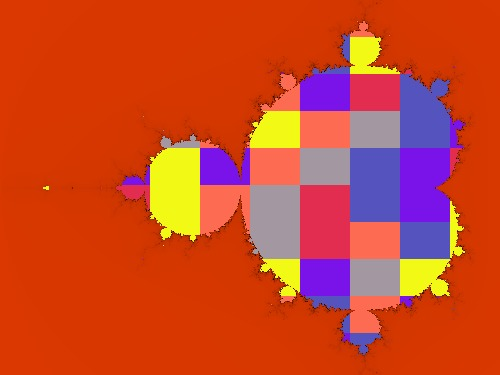
\includegraphics[scale=0.4]{figurer/loadbalance.jpg}
	\end{center}
	\caption{Loadbalanced implementation.}
	\label{fig:loadbalance}
\end{figure}

\begin{figure}[H]
	\begin{center}
		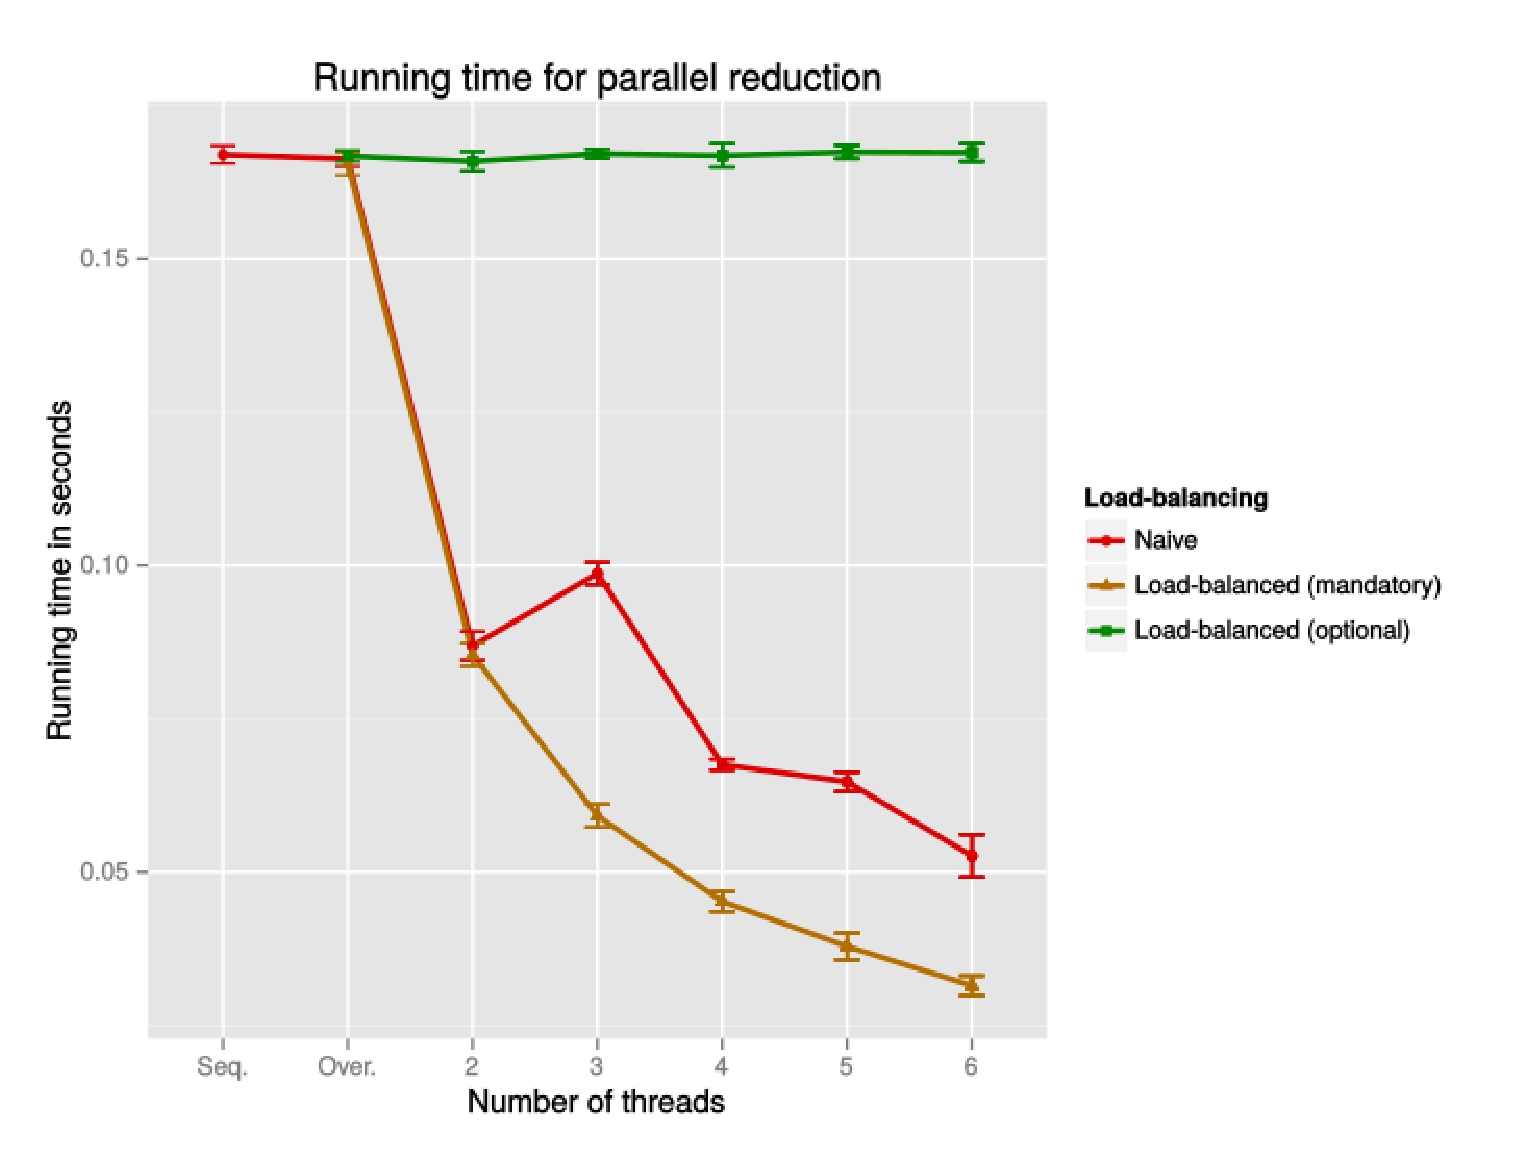
\includegraphics[scale=0.3]{figurer/both_time.eps}
	\end{center}
	\caption{Running time for both implementations.}
	\label{fig:both_time}
\end{figure}

\begin{figure}[H]
	\begin{center}
		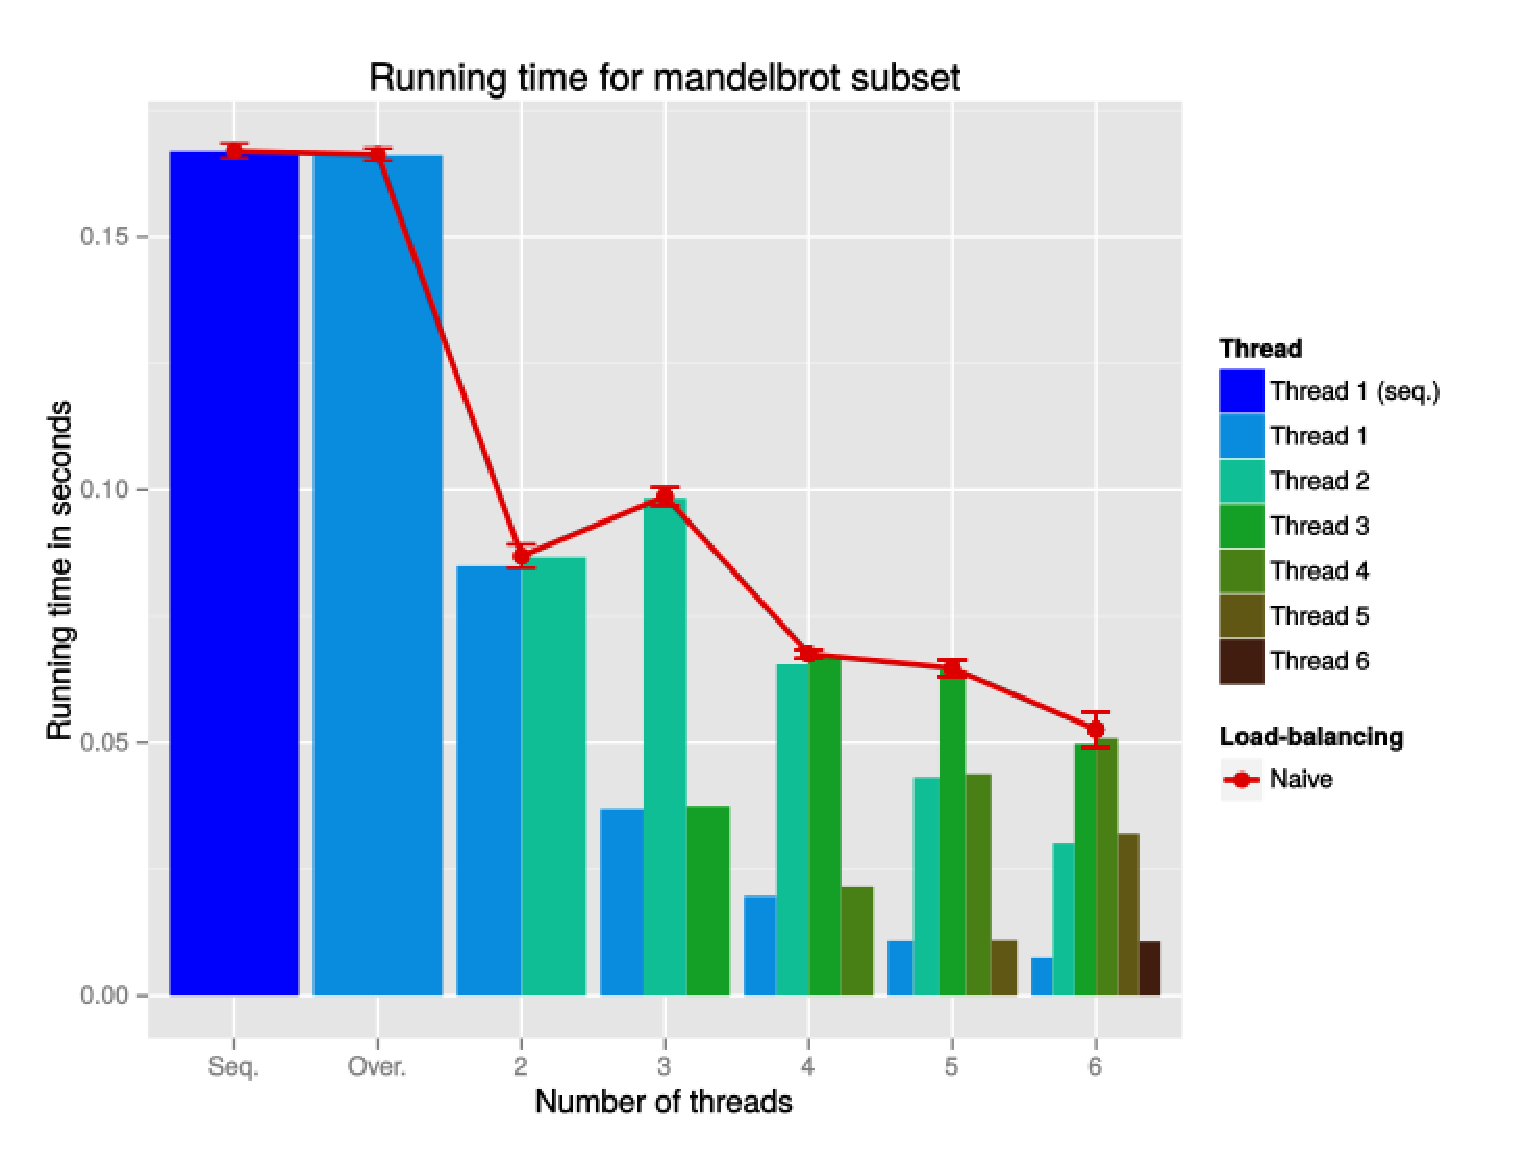
\includegraphics[scale=0.3]{figurer/naive_time.eps}
	\end{center}
	\caption{Naive work distribution.}
	\label{fig:naive_time}
\end{figure}

\begin{figure}[H]
	\begin{center}
		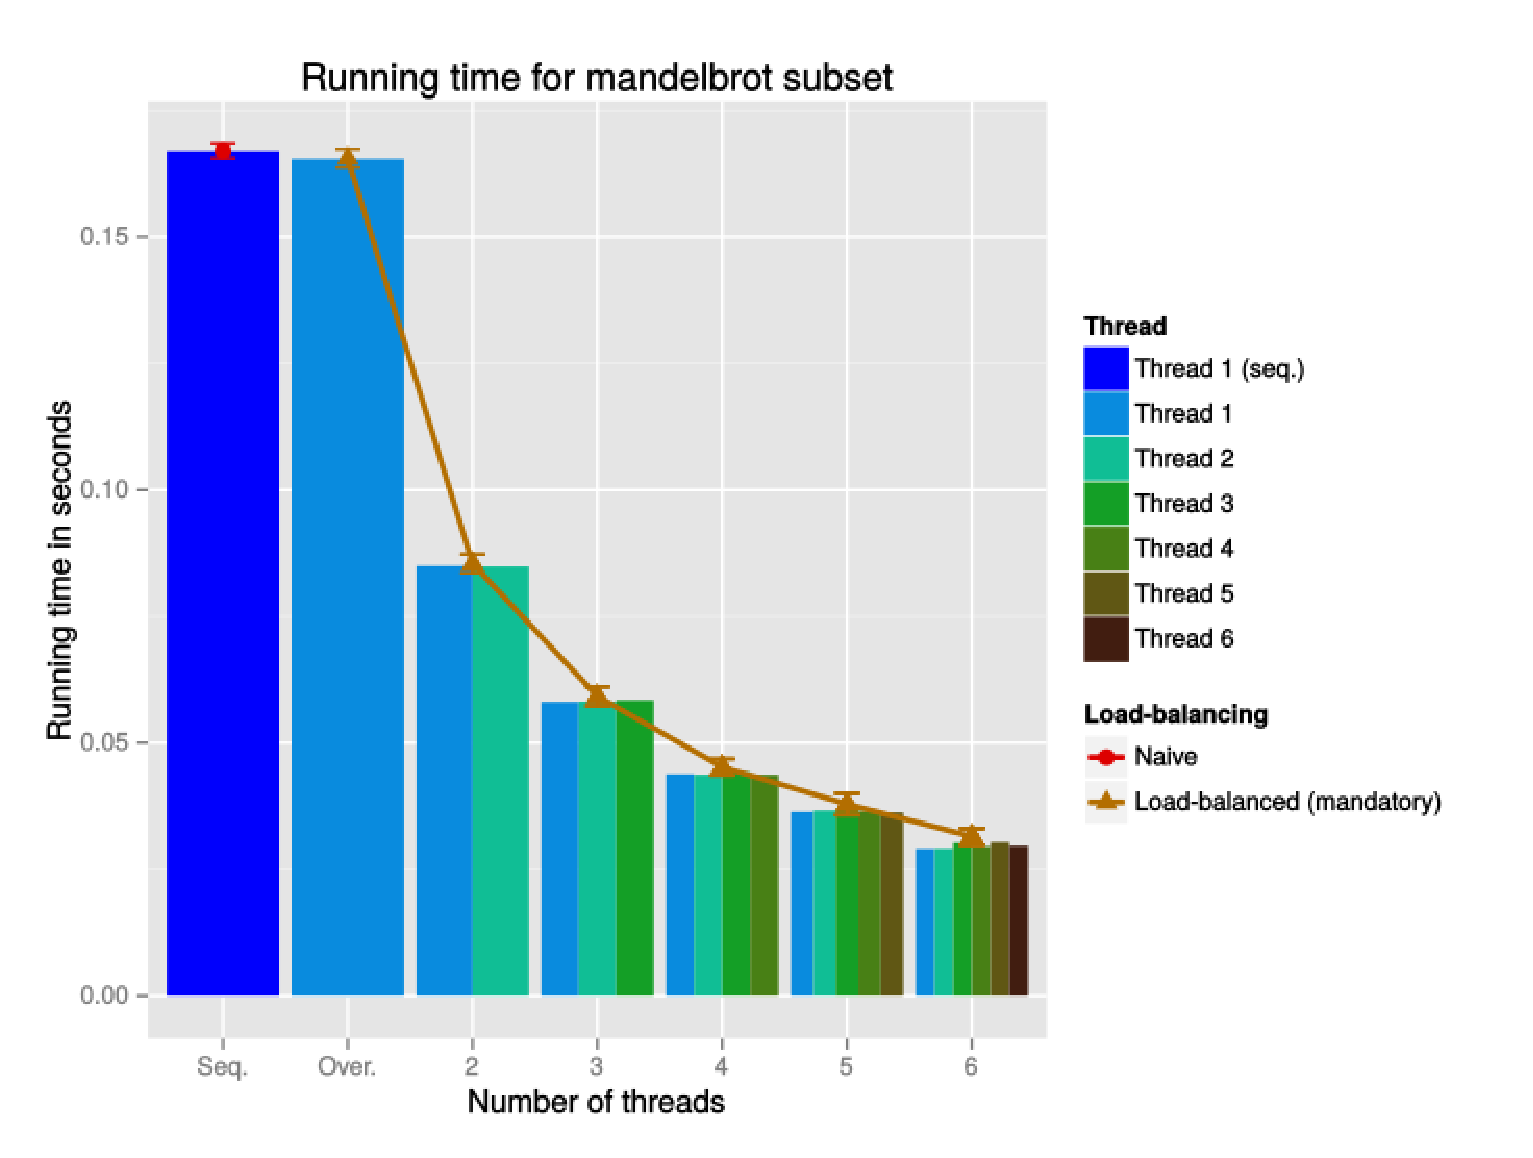
\includegraphics[scale=0.3]{figurer/loadbalance_time.eps}
	\end{center}
	\caption{Loadbalanced work distribution.}
	\label{fig:loadbalance_time}
\end{figure}


\newpage

\onecolumn
\appendix
\section{Naive implementation} \label{app:naive}
\lstinputlisting[language=c]{matlab/naive.c}
\section{Loadbalanced implementation} \label{app:loadbalance}
\lstinputlisting[language=c]{matlab/loadbalance.c}
\end{document}
